
\tikzset{every picture/.style={line width=0.75pt}} %set default line width to 0.75pt

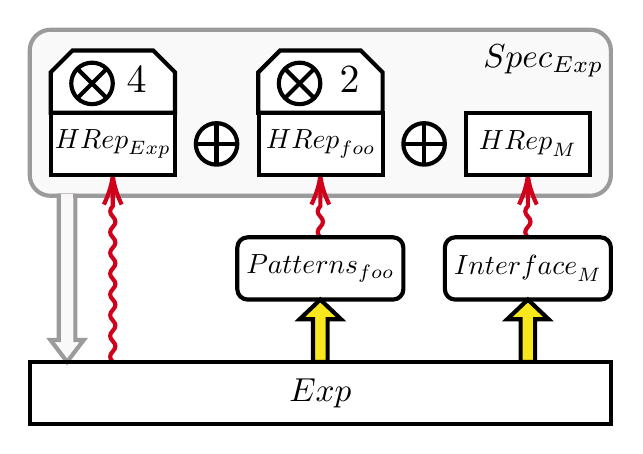
\begin{tikzpicture}[x=0.75pt,y=0.75pt,yscale=-1,xscale=1]
%uncomment if require: \path (0,416.5); %set diagram left start at 0, and has height of 416.5

%Shape: Rectangle [id:dp9489660675592899]
\draw  [color={rgb, 255:red, 155; green, 155; blue, 155 }  ,draw opacity=1 ][fill={rgb, 255:red, 249; green, 249; blue, 249 }  ,fill opacity=1 ][line width=1.5]  (130,20) .. controls (130,14.48) and (134.48,10) .. (140,10) -- (400,10) .. controls (405.52,10) and (410,14.48) .. (410,20) -- (410,80) .. controls (410,85.52) and (405.52,90) .. (400,90) -- (140,90) .. controls (134.48,90) and (130,85.52) .. (130,80) -- cycle ;
%Snip Same Side Corner Rect [id:dp09931070350524518]
\draw  [fill={rgb, 255:red, 255; green, 255; blue, 255 }  ,fill opacity=1 ][line width=1.5]  (140.1,30.5) -- (150.6,20) -- (189.5,20) -- (200,30.5) -- (200,50) -- (200,50) -- (140.1,50) -- (140.1,50) -- cycle ;
%Down Arrow [id:dp5984296172784]
\draw  [color={rgb, 255:red, 155; green, 155; blue, 155 }  ,draw opacity=1 ][fill={rgb, 255:red, 249; green, 249; blue, 249 }  ,fill opacity=1 ][line width=1.5]  (140,159.5) -- (144,159.5) -- (144,90) -- (152,90) -- (152,159.5) -- (156,159.5) -- (148,170) -- cycle ;
%Straight Lines [id:da30879479079788386]
\draw [color={rgb, 255:red, 249; green, 245; blue, 245 }  ,draw opacity=1 ][fill={rgb, 255:red, 249; green, 249; blue, 249 }  ,fill opacity=1 ][line width=1.5]    (145,90) -- (151,90) ;


%Straight Lines [id:da5824111707250128]
\draw [color={rgb, 255:red, 208; green, 2; blue, 27 }  ,draw opacity=1 ][line width=1.5]    (170,170) .. controls (168.33,168.33) and (168.33,166.67) .. (170,165) .. controls (171.67,163.33) and (171.67,161.67) .. (170,160) .. controls (168.33,158.33) and (168.33,156.67) .. (170,155) .. controls (171.67,153.33) and (171.67,151.67) .. (170,150) .. controls (168.33,148.33) and (168.33,146.67) .. (170,145) .. controls (171.67,143.33) and (171.67,141.67) .. (170,140) .. controls (168.33,138.33) and (168.33,136.67) .. (170,135) .. controls (171.67,133.33) and (171.67,131.67) .. (170,130) .. controls (168.33,128.33) and (168.33,126.67) .. (170,125) .. controls (171.67,123.33) and (171.67,121.67) .. (170,120) .. controls (168.33,118.33) and (168.33,116.67) .. (170,115) .. controls (171.67,113.33) and (171.67,111.67) .. (170,110) .. controls (168.33,108.33) and (168.33,106.67) .. (170,105) .. controls (171.67,103.33) and (171.67,101.67) .. (170,100) .. controls (168.33,98.33) and (168.33,96.67) .. (170,95) -- (170,91) -- (170,83) ;
\draw [shift={(170,80)}, rotate = 450] [color={rgb, 255:red, 208; green, 2; blue, 27 }  ,draw opacity=1 ][line width=1.5]    (14.21,-4.28) .. controls (9.04,-1.82) and (4.3,-0.39) .. (0,0) .. controls (4.3,0.39) and (9.04,1.82) .. (14.21,4.28)   ;

%Straight Lines [id:da7051587981224026]
\draw [color={rgb, 255:red, 208; green, 2; blue, 27 }  ,draw opacity=1 ][line width=1.5]    (270,110) .. controls (268.33,108.33) and (268.33,106.67) .. (270,105) .. controls (271.67,103.33) and (271.67,101.67) .. (270,100) .. controls (268.33,98.33) and (268.33,96.67) .. (270,95) -- (270,91) -- (270,83) ;
\draw [shift={(270,80)}, rotate = 450] [color={rgb, 255:red, 208; green, 2; blue, 27 }  ,draw opacity=1 ][line width=1.5]    (14.21,-4.28) .. controls (9.04,-1.82) and (4.3,-0.39) .. (0,0) .. controls (4.3,0.39) and (9.04,1.82) .. (14.21,4.28)   ;

%Straight Lines [id:da6087008244886778]
\draw [color={rgb, 255:red, 208; green, 2; blue, 27 }  ,draw opacity=1 ][line width=1.5]    (370,110) .. controls (368.33,108.33) and (368.33,106.67) .. (370,105) .. controls (371.67,103.33) and (371.67,101.67) .. (370,100) .. controls (368.33,98.33) and (368.33,96.67) .. (370,95) -- (370,91) -- (370,83) ;
\draw [shift={(370,80)}, rotate = 450] [color={rgb, 255:red, 208; green, 2; blue, 27 }  ,draw opacity=1 ][line width=1.5]    (14.21,-4.28) .. controls (9.04,-1.82) and (4.3,-0.39) .. (0,0) .. controls (4.3,0.39) and (9.04,1.82) .. (14.21,4.28)   ;

%Shape: Rectangle [id:dp701556783783656]
\draw  [line width=1.5]  (230,115) .. controls (230,112.24) and (232.24,110) .. (235,110) -- (305,110) .. controls (307.76,110) and (310,112.24) .. (310,115) -- (310,135) .. controls (310,137.76) and (307.76,140) .. (305,140) -- (235,140) .. controls (232.24,140) and (230,137.76) .. (230,135) -- cycle ;

%Shape: Rectangle [id:dp033430127809365384]
\draw  [line width=1.5]  (330,115) .. controls (330,112.24) and (332.24,110) .. (335,110) -- (405,110) .. controls (407.76,110) and (410,112.24) .. (410,115) -- (410,135) .. controls (410,137.76) and (407.76,140) .. (405,140) -- (335,140) .. controls (332.24,140) and (330,137.76) .. (330,135) -- cycle ;
%Shape: Rectangle [id:dp6050538306488522]
\draw  [fill={rgb, 255:red, 255; green, 255; blue, 255 }  ,fill opacity=1 ][line width=1.5]  (140.1,50) -- (200,50) -- (200,80) -- (140.1,80) -- cycle ;
%Shape: Rectangle [id:dp9303311048687424]
\draw  [fill={rgb, 255:red, 255; green, 255; blue, 255 }  ,fill opacity=1 ][line width=1.5]  (340,50) -- (400,50) -- (400,80) -- (340,80) -- cycle ;

%Up Arrow [id:dp0013771056350821986]
\draw  [color={rgb, 255:red, 0; green, 0; blue, 0 }  ,draw opacity=1 ][fill={rgb, 255:red, 248; green, 231; blue, 28 }  ,fill opacity=1 ][line width=1.5]  (260,149.5) -- (270,140) -- (280,149.5) -- (273.5,149.5) -- (273.5,170) -- (266.5,170) -- (266.5,149.5) -- cycle ;
%Shape: Rectangle [id:dp7366907361635939]
\draw  [fill={rgb, 255:red, 255; green, 255; blue, 255 }  ,fill opacity=1 ][line width=1.5]  (240.43,50) -- (300,50) -- (300,80) -- (240.43,80) -- cycle ;
\draw  [fill={rgb, 255:red, 255; green, 255; blue, 255 }  ,fill opacity=1 ][line width=1.5]  (210,65) .. controls (210,59.48) and (214.48,55) .. (220,55) .. controls (225.52,55) and (230,59.48) .. (230,65) .. controls (230,70.52) and (225.52,75) .. (220,75) .. controls (214.48,75) and (210,70.52) .. (210,65) -- cycle ; \draw  [line width=1.5]  (210,65) -- (230,65) ; \draw  [line width=1.5]  (220,55) -- (220,75) ;
\draw  [fill={rgb, 255:red, 255; green, 255; blue, 255 }  ,fill opacity=1 ][line width=1.5]  (310,65) .. controls (310,59.48) and (314.48,55) .. (320,55) .. controls (325.52,55) and (330,59.48) .. (330,65) .. controls (330,70.52) and (325.52,75) .. (320,75) .. controls (314.48,75) and (310,70.52) .. (310,65) -- cycle ; \draw  [line width=1.5]  (310,65) -- (330,65) ; \draw  [line width=1.5]  (320,55) -- (320,75) ;
\draw  [fill={rgb, 255:red, 255; green, 255; blue, 255 }  ,fill opacity=1 ][line width=1.5]  (152.93,28.79) .. controls (156.83,24.88) and (163.17,24.88) .. (167.07,28.79) .. controls (170.98,32.69) and (170.98,39.02) .. (167.07,42.93) .. controls (163.17,46.83) and (156.83,46.83) .. (152.93,42.93) .. controls (149.02,39.02) and (149.02,32.69) .. (152.93,28.79) -- cycle ; \draw  [line width=1.5]  (152.93,28.79) -- (167.07,42.93) ; \draw  [line width=1.5]  (167.07,28.79) -- (152.93,42.93) ;
%Snip Same Side Corner Rect [id:dp4221187902899477]
\draw  [fill={rgb, 255:red, 255; green, 255; blue, 255 }  ,fill opacity=1 ][line width=1.5]  (240.1,30.5) -- (250.6,20) -- (289.5,20) -- (300,30.5) -- (300,50) -- (300,50) -- (240.1,50) -- (240.1,50) -- cycle ;
\draw  [fill={rgb, 255:red, 255; green, 255; blue, 255 }  ,fill opacity=1 ][line width=1.5]  (252.93,28.79) .. controls (256.83,24.88) and (263.17,24.88) .. (267.07,28.79) .. controls (270.98,32.69) and (270.98,39.02) .. (267.07,42.93) .. controls (263.17,46.83) and (256.83,46.83) .. (252.93,42.93) .. controls (249.02,39.02) and (249.02,32.69) .. (252.93,28.79) -- cycle ; \draw  [line width=1.5]  (252.93,28.79) -- (267.07,42.93) ; \draw  [line width=1.5]  (267.07,28.79) -- (252.93,42.93) ;
%Shape: Rectangle [id:dp1692119124811613]
\draw  [line width=1.5]  (130,170) -- (410,170) -- (410,200) -- (130,200) -- cycle ;
%Up Arrow [id:dp4999372801455]
\draw  [color={rgb, 255:red, 0; green, 0; blue, 0 }  ,draw opacity=1 ][fill={rgb, 255:red, 248; green, 231; blue, 28 }  ,fill opacity=1 ][line width=1.5]  (360,149.5) -- (370,140) -- (380,149.5) -- (373.5,149.5) -- (373.5,170) -- (366.5,170) -- (366.5,149.5) -- cycle ;

% Text Node
\draw (270,185) node [scale=1.2]  {$Exp$};
% Text Node
\draw (270,125) node [scale=1]  {$\text{Patterns}_{foo}$};
% Text Node
\draw (370,125) node [scale=1]  {$\text{Interface}_{M}$};
% Text Node
\draw (170.05,65) node [scale=1]  {$\text{HRep}_{Exp}$};
% Text Node
\draw (370,65) node [scale=1]  {$\text{HRep}_{M}$};
% % Text Node
% \draw (77.5,125) node [scale=1.2]  {$Spec_{Exp}\Downarrow \ Exp$};
% Text Node
\draw (377.5,25) node [scale=1.2]  {$Spec_{Exp}$};
% Text Node
\draw (270.22,65) node [scale=1]  {$\text{HRep}_{foo}$};
% Text Node
\draw (181.5,34) node [scale=1.44]  {$4$};
% Text Node
\draw (284.05,34) node [scale=1.44]  {$2$};


\end{tikzpicture}
